\documentclass{article}

\usepackage{subcaption}
\usepackage{graphicx}
\usepackage{amsmath}
\usepackage{color}
\usepackage{fullpage}
\usepackage{pgfgantt}
\usepackage{booktabs}
\usepackage{tabularx}
\usepackage{relsize}
\usepackage{epigraph}
\usepackage{parskip}
\usepackage{float}
\usepackage{listings}
\usepackage{tcolorbox}
\usepackage{algorithm}
\usepackage{algpseudocode}
\usepackage{pgfplots}

\renewcommand{\familydefault}{\sfdefault}

\definecolor{pr0}{RGB}{61, 255, 12}
\definecolor{pr1}{RGB}{208, 231, 11}
\definecolor{pr2}{RGB}{255, 190, 0}
\definecolor{pr3}{RGB}{231, 149, 11}
\definecolor{pr4}{RGB}{255, 95, 6}
\definecolor{pr5}{RGB}{231, 20, 3}
\definecolor{pr6}{RGB}{255, 12, 190}

\definecolor{codeblue}{HTML}{528bff}
\definecolor{codegreen}{HTML}{98C379}
\definecolor{codepurple}{HTML}{C678DD}
\definecolor{codebg}{gray}{0.92}

\newtcbox{\codeinline}{nobeforeafter,colframe=codebg,colback=codebg,arc=1pt,boxrule=0.5pt, left=0.5pt,right=0.5pt,top=0.5pt,bottom=0.5pt,tcbox raise base}

\newcommand{\code}[1]{\codeinline{\texttt{#1}}}

\lstdefinestyle{cpp}{
  language=C++,
  basicstyle=\ttfamily,
  backgroundcolor=\color{codebg},
  numberstyle=\color{black},
  keywordstyle=\color{codeblue},
  commentstyle=\color{codegreen},
  stringstyle=\color{codepurple},
  breakatwhitespace=false,
  breaklines=true,
  columns=flexible,
  keepspaces=true,
  firstnumber=1,
  numbers=left,
  numbersep=3pt,
  tabsize=4,
  title=\lstname
}

\lstset{escapechar=@,style=cpp}

\title{Senior Project Thesis\\
  \large Process scheduling - comparison and contrast}
\date{\today}
\author{Martin Nestorov}
\linespread{1}

\begin{document}

\maketitle
\pagenumbering{arabic}

\newpage

\section{\underline{Introduction}}

Every Operating System has some type of process handling capabilities, be that in the form of simple queue structure, or in some complex algorithm. This is also specific to the different types of systems that are handling the jobs. Some embedded systems do not have the capacity to handle complex operations, which forces them to have simple schedulers. One such example would be preemptive OS's, running on batch jobs.

There are several process scheduling algorithms that are used in batch, interactive, and real-time systems. These include, but are not limited to, First Come First Serve (\textbf{FCFS}), Shortest Job First (\textbf{SJF}), Priority Job First (\textbf{PJF}), \textbf{Round-Robin} Scheduling, Guaranteed Scheduling, Lottery Scheduling, \textbf{Multilevel Queue} Scheduling, etc. All of them have their advantages and weaknesses. Some are simpler and work for small systems, while others are more complex, but distribute the workload better. The purpose of this project is to analyze and compare these different algorithms, to show where they flourish and where they fall.

Another thing to consider is the type of the system that lies under the processes. In general, we can either consider a \textit{Real-time} system, or an \textit{Interactive} one. We are all together omitting \textit{Batch} systems, as they are no longer viable and interesting. \textit{Real-time} systems are such that take into consideration time as an essential goal. Typically, one or more devices can stimulate the system and it has to react accordingly in a certain amount of time. \textit{Interactive} systems, much like the 'Real-time' ones, can and are stimulated by other programs, but don't have such a strict time constraints.

I personally find the topic of these intricate systems fascinating. All of these schedulers have something to teach us about optimization and managing complex systems. Being able to control an entire Operating Systems is no joke, so a good handle on \textit{Process Scheduling Algorithms} is vital for any Computer Scientist. As I aspire to one day write kernel code, this project closely relates to my interests and is a good preparation for any further advancements in the fields of \textit{System programming}. Although this project is big in size and complexity, the desire to learn proves to justify any means to achieve the goal.

\epigraph{He who has a why to live can bear almost any how}{\textit{Friedrich Nietzsche}}

The application is created by using \code{C++} and the \code{ncurses} library. The reason to pick \textit{C++} is due to its high granularity and fine tuning capabilities. With C++, I can control every aspect of the program with high accuracy, which is needed for scheduling algorithms. The \textit{ncurses} library provides a nice platform for building \textit{terminal-based} applications. It allows for easy interaction with terminals, controlling text output, color output, \textit{IO} operations, etc. It also provides a clean and pretty \textit{user-interface}, which is always a welcome benefit, especially if the work is done in C++. The \textit{UI} will have several panels, indicating the different algorithms and processes that can be selected, and also what are the contents of the different \code{queues}. There would be information for each algorithm and statistical summaries after each round of execution. The UI aims at being both easy to use, but at the same time, be clear and helping people evaluate the different algorithms.

As a final goal, this project is to be shared and extended with anyone who is interested in learning the mechanics of process scheduling. It can be used as a learning and pedagogical tool. Future plans hold that the project be tailored for introductory courses on Operating Systems, where students will have a first hand experience of seeing how these algorithms work and what kind of outputs they produce. This means that the project should be able to compile on multiple machines, which are at least capable of supporting \code{C++ 11} and \code{ncurses}.

\begin{figure}[H]
  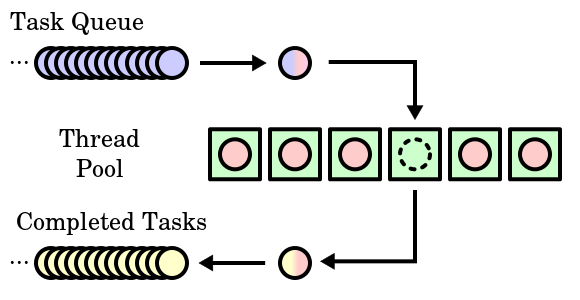
\includegraphics[width=\linewidth]{./pics/thread_pool.png}
  \caption{Thread Pool}
  \label{fig:Thread Pool}
\end{figure}

This diagram shows us the most basic and fundamental way to treat a process scheduling system. It's just a queue with tasks, inserted into a Thread Pool, which then picks one of the many tasks (or jobs), executes them, and sends them to the Complete Queue. Rinse and repeat.

\section{\underline{Specification and Analysis of the Software Requirements}}

\subsection{Requirements}

This software has a set of requirements that have to be met and covered in order to be held as working and complete, before it can be released for any pedagogical or personal usage. These specifications are separated into \textit{functional} and \textit{non-functional} requirements. The aim of the functional requirements is to describe what the software \textbf{should do}. Most of them aim at simplicity and ease of use of the application. The non-functional, on the other hand, try to provide a fast, extensible and stable experience to the user.

First, let's start with the analysis of the functional requirements. The software \textit{should}:

\begin{itemize}
\item \textit{Having a simple and readable user interface}. This means that all of the panels in the program should be easy to understand and differentiate between one another. Things like clear panel headlines, obvious execution patters, proper color coding of processes and commands, are a \textbf{must}. Each process should and will be assigned a priority either manually or automatically, but regardless, for each one, there should be a corresponding color that would give a general indication as to what that process's priority is. This goes hand in hand with how each process will be displayed in the different panels during execution. Because there will be commands that will create processes manually, each one should be clear, both with text and with color, what type of process is about to be created. In addition to the readability of the project, appropriate textual information should be given for each algorithm that is currently running. In the panel \textbf{Legend}, where all of this information will be held, a brief description of each action should be given, so that anyone who is executing an algorithm knows what is happening. Because this project will also be dynamically executing processes, it should also inform the user at each step what is happening. This means that the project should have a stable state at each moment and that the user knows it. This can be achieved through either labels or headings clearly shown in color at every moment.

\item \textit{Respond to all types of inputs}. One of the more complicated software aspects of this project is the responsiveness. Each process can executed for varying times, which means that the user might wait for one second or more, and although this is the normal behavior of the application, it should be made clear to the user that this is happening. With that, the user should be restricted to the commands and inputs he/she can do at any moment. The application is build to be light and fast, but it also has to handle every response from the \textit{UI}. This means that when an invalid character is submitted from the keyboard, the program should not be affected by it and should continue working. When a valid character is sent, the affects of that should also be made clear and responsive. Thus robustness is ensured for all users.

\item \textit{Be able to compare and analyze produced data}. Because this project has a purpose to evaluate and compare different algorithms, it should be made easy to have a set of saved \textit{already executed} processes and what their evaluation is. Thus, for each execution, every time and algorithm is executed, it should be saved for further evaluation and should be made easily readable by anyone. Then the last 10 executions and their summaries should be put on the screen when the user enters the appropriate command and wants to see and compare them. Finally, these summaries should be saved to a text file so that they can be separately analyzed if needed. Although only the last 10 executions will be shown, all of the previously run algorithms should be saved no matter what.
\end{itemize}

And here are some of the non-functional requirements. They focus on usability, efficiency, quality, speed, etc. These things focus on \textbf{how} the software \textit{should}:

\begin{itemize}
\item \textit{Create completely random processes}. Each process can either be created with a \textit{pre-defined} priority, or with an automatically set one (i.e. on a random principle). The processes that are randomly generated should be properly distributed and should not follow a pattern in any way. The need for such a requirement ensures that there are no hidden rules or patterns that would disrupt the evaluations and comparisons later on. That is why there has to be a proper distribution of processes with their values. For each process, the \code{ID} should be randomly generated to be a hexadecimal number with an even distribution between all processes, the \code{ttl} (time to live) should correspond to a \textit{Gaussian Distribution} with a predefined mean and standard deviation. The same should also apply to every \textit{IO} operation and their quantity.

\item \textit{Have high code quality}. Software craftsmanship is highly valued. It's expected that after the end of the project, maintenance and further improvements will be continually made, especially if the project is to be used for teaching purposes. If the code is not structured and prepared in such a way, that allows for further expansions and easy bug-fixing, then that would provide for a poor project life. This means that the code base should have correct comment sections, code documentation above each method, perfect separation of concerns, a valid architectural model that is followed to the end, diagrams that help understand the project and a list of future works to be done. If this is not met, then neither the original creator, nor any following contributor would want to maintain this software and any piece of code that is not regularly maintained, falls of the market and becomes useless.

\item \textit{Non-intrusive help from the User Interface}. It is very important that any form of help that comes from the system to be as inconspicuous as possible. User friendliness is achieved when the user thinks he/she have discovered something on their own. This should be done through layered error messages, that are generated on each step of processing, allowing for a decoupled, yet understandable explanation of the situation. In addition to this, all of the helper functions should have hints as to how to make the functionality of the project more approachable.
\end{itemize}

\underline{\textbf{Constraints}}

The application should \textbf{not} try to implement every algorithm for scheduling and have a \(1:1\) correspondence with real-life systems used in production. It should try to get as possible in order to do proper analysis and evaluation, without falling into the pit of meticulous pedantic, which are not worth implementing. This does not mean to restrict the number of algorithms, or to limit it to the most simple ones, but to put a realistic boundary on what should be expected from this product. A good mixture of complexity and quantity would fit the bill perfectly.

\subsection{\underline{Use cases}}

This project is targeted at two general use groups. One group is for those who want to test and examine scheduling algorithms, see how they work and how they present themselves in a graphical way. The other group is for people who want to learn and have a learning experience in the world of operating systems. In some sense, this project can be seen as either a research tool, or as a pedagogical tool. In both cases we see how different process scheduling algorithms work underneath the hood and see how to compare their abilities. For people who want to learn or get a better idea as to why systems are working the way they are, through running the application and looking at the source code, this project is a great place for research and learning.

\begin{figure}[H]
  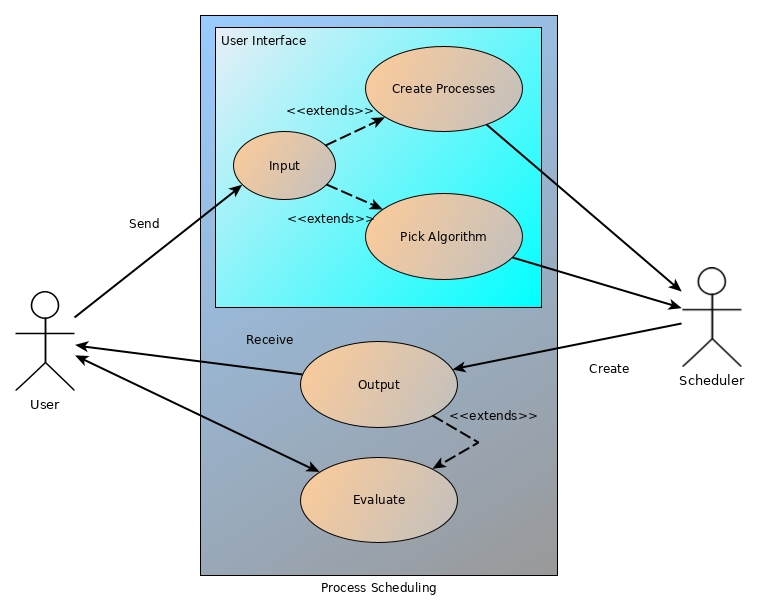
\includegraphics[width=\linewidth]{./pics/usecase.jpg}
  \caption{Use-Case Diagram}
  \label{fig:Use-Case Diagram}
\end{figure}

This use case diagram can help us understand how exactly to use the application. We can see that the actor in the picture would be anyone who is using the application. Because this application is not an online service, the usage is controlled solely by the user. First, the student or researcher interacts with User Interface of the app, which is part of the graphical layer. Through it, the actor is able to create different processes, where each one will be used to run in the demo algorithm. Then after the process creation is done, the actor picks the desired algorithm and then the control of the app is handed to the Scheduler component. In this diagram, we can treat the Scheduler as another actor, because it is providing a certain type of service and is giving output in the end. After the algorithm has finished, a summary in the form of an output is given to the user. Then the user, if he/she wishes, can evaluate the received results.

\begin{figure}[H]
  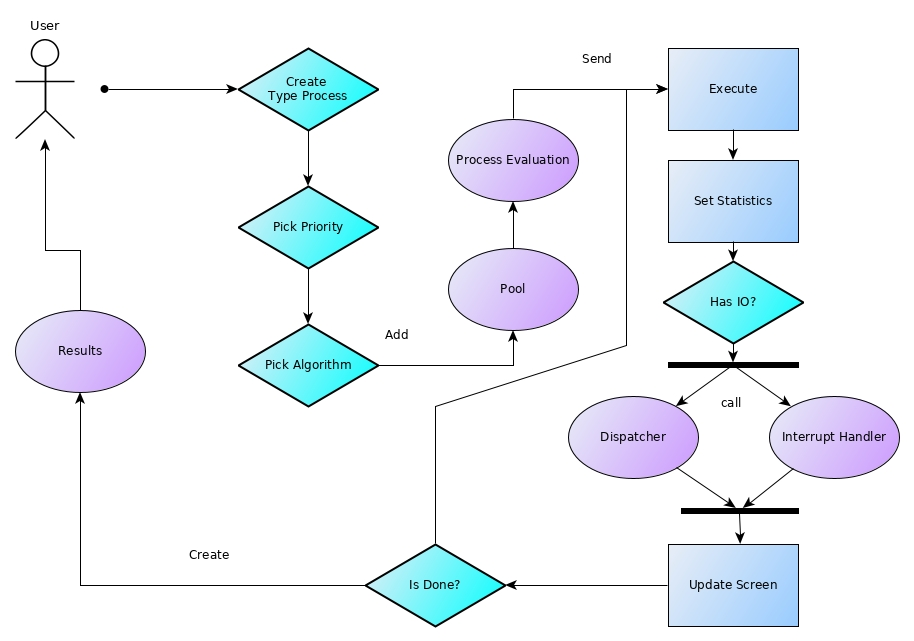
\includegraphics[width=\linewidth]{./pics/activity.jpg}
  \caption{Activity Diagram}
  \label{fig:Activity Diagram}
\end{figure}

In this Activity Diagram, we can see in detail the different steps that are taken at each moment for the creating and execution of each algorithm. First, we start with a few choices that influence the processes we will see in the app. Namely, these are the priorities that each process will have. After that, an algorithm is picked. We notice here that we first have to create processes and assign them priorities, because otherwise the algorithm will be working on an empty pool of processes, which makes no sense. After that, we go to the pool entity of the program and we evaluate each processes based on the total execution time it has. If the processes, however, does have a predefined priority, we do not override it. This means that this evaluation is done for randomly created processes, and that's okay.

After this step, we then move on to the execution of the picked algorithm. The procedure here is such that we first do the "empty" work on each process and then evaluate the needed statistics for each process, then we check through a method if that process will get into an IO state or not. Based on that, we either call the dispatcher part of the procedure or the interrupt handler. If the dispatcher is called, then we do context switch and we continue with the next process. If the interrupt handler is called, then we create a separate thread that executes the IO operations.

In the end, we update the screen with all of this information and we check if the process is done. If it is not, then we just loop back to the pool and star all over until the whole pool is executed completely. If it is however, then we finish everything and give the desired output to the user!

\begin{figure}[H]
  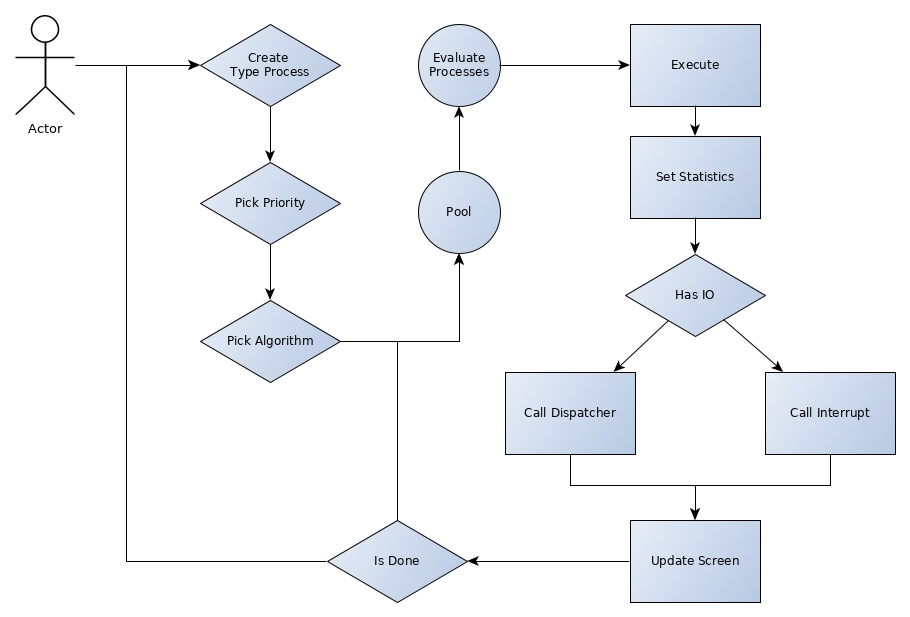
\includegraphics[width=\linewidth]{./pics/pipeline.jpg}
  \caption{Pipeline Diagram}
  \label{fig:Pipeline Diagram}
\end{figure}

Additionally, we also have a pipeline diagram that shows us what is the general procedure of each run of the application. Through this, we can see what each part of the program does and in what context it is. First, we see that we have a process creation step, that is concerned with populating the pool of processes. For each input, we create a process and assign it a priority, either manually or automatically. Then we pick the algorithm we want to see running. All of this information is sent to the global pool of processes. We can see that the pool holds in itself all of the processes. While this is happening, we can evaluate the processes by priority, based on their execution time. We do this right before we start the main algorithm execution. When we start that part, we move each process from the ready queue into the execution step. We pick which process to move based on the selected algorithm. Then we execute the picked process for some amount of time, also dependent on the selected algorithm. When this is done, we add the statistical data that this execution has accumulated and then we check if we have to do any IO operations. Depending on that answer, we either call the Dispatcher or the Interrupt Handler. If we call the Dispatcher, then we do a context switch, otherwise, we execute the IO operation waiting next. In the end, we check if the process is done or not. Until there are still unfinished processes, we get the next one and loop right back to the execution step. When everything is finished, we move the processes to the done queue and then update the screen and create the result, which is sent to the user.

\section{\underline{Design of the Software Solution}}

This software uses several algorithms and data-structures that play a key role in the whole inner-workings. Because the purpose of the project is to show how different algorithms affect the process execution of \textit{Real-Time} systems, we have to talk about each used algorithm and the accompanying data-structures.

But before we do that, we have to cover several structural decisions that have been made in order for the algorithm explanations to make sense.

Usually, in scheduling algorithms we have \code{PCB} blocks which hold references to the actual process, and through those blocks, we make decisions on which process should be executed next. Instead of doing this, because it adds another layer of complexity, not needed in this case, the role of a process and a PCB block is substituted with just a \code{process} class. It holds both the metadata found in PCBs and has the workings of processes. Thus, when in the text a reference is made to a process, a mental note should be made that it has a duality in it, for it holds two structures. The explanation of the \code{process} structure, as well as the other classes, can be found further down.

Another aspect that should be considered is that this project tries to imitate a \textit{Real-Time} system. This means that the scheduler has the notion of preemptive tasks and of \textit{IO} operations. Some of algorithms used are non-primitive and have been used in old \textit{batch systems} and \textit{interactive systems}. Thus, these algorithms have been tailored in order to work with a modern approach of building schedulers. When we refer to preemptive systems, it is meant that the OS decides when a process should be forced into a context-switch and when it should be taken from the \code{ready\_queue}. Also, Real Time systems do not wait for IO to end, thus they switch to the next ready process. For instance, the \textbf{FCFS} algorithm originally was used in non-preemptive batch systems, but in this project, each process is preempted upon requesting IO operations. Then, while waiting for that process to finish with IO, the next ready one is taken from the queue.

Having these distinctions made, we can then proceed to the algorithms and data-structures used.

\subsection{\underline{Algorithms and Data-structures}}

\subsubsection{\underline{FCFS}}

The \textbf{F}irst \textbf{C}ome \textbf{F}irst \textbf{S}erve algorithm is one of the easiest to understand and implement. It can be looked at from many different angles. \textbf{FCFS} can be seen as a \code{linked-list} or a \code{queue}, which just serves each incoming process to the CPU for execution. When a new process is created, it is put at the back of the \code{ready\_queue}. Then each process, one by one, is taken from the head of the queue and is given to the CPU for execution. It really depends on what type of system is running this scheduler, but in general, this algorithm, although easy, is not the most effective one to have. Because each process can take any time to finish, it can stall the whole system with its execution. For instance, if we were to have several processes and one is to be long in execution time, depending on their time of arrival, we can either quickly go through all of them, or we can wait for a long time.

In this project, the \textbf{FCFS} algorithm is created using a \code{vector} to hold all of the processes in sequential manner. At the start of the algorithm, we just take each next process for execution, wait for its time to live (\code{ttl}) and then we proceed to the next one in line. Because this project tries to imitate a \textit{Real-Time} system, we also check if each process will do an \textit{IO} operation. If so, the process is then sent to an \code{exec\_io} routine, and the next process is then taken. This means that the \code{done\_queue} will not be populated in the exact same order as the processes have been created in the \code{ready\_queue}, because of these \textit{IO} operations. Regardless, this still follows the \textbf{FCFS} pattern, and we can see that indeed, each process is taken from the head of the queue (technically vector).

\bigskip

\underline{\textbf{Evaluation}}

\textbf{FCFS} gives us a few benefits. First, it is very simple to implement and understand. From this standpoint, it's a great algorithm for small batch systems. But on the other hand, it doesn't scale well. It can stall if there is \textbf{no} preemption and a \textbf{convoy effect} might occur, which means that all other processes wait for the currently running one to finish. To summarize:

\begin{table}[H]
  \begin{tabularx}{\linewidth}{>{\parskip1ex}X@{\kern4\tabcolsep}>{\parskip1ex}X}
    \toprule
    \hfil\bfseries Pros & \hfil\bfseries Cons \\
    \cmidrule(r{3\tabcolsep}){1-1}\cmidrule(l{-\tabcolsep}){2-2}

    Easy to implement\par
    Easy to understand\par
    Works good for simple systems and batch systems\par

    &

    Can be slow\par
    Doesn't scale\par
    High risk of convoy effect\par
    System can stall if not preemptive\par
    Bad prediction for \textit{Waiting time} and \textit{Turnaround time} \\
    \bottomrule
    \toprule
    \hfil\bfseries Algorithm Complexity & \hfil\bfseries Execution Complexity \\

    \\
    \centerline{$O(n)$}\par

    &

    \centerline{$O(n)$}
  \end{tabularx}
  \caption{Pros and Cons of FCFS}
\end{table}

From this table we can also see how the complexity of the algorithm together with its execution complexity align. The reason that FCFS is in linear time when it comes to the algorithm complexity is because we are iterating over the whole bunch of processes in the pool. We are doing that in a sequential manner, meaning that we would not be skipping over anything. This is fine, but when we look at the execution complexity, we can see that we also have linear time. This is not the most optimal complexity we can have, because we are going through every process and we are also blocking the CPU, if that process has a long execution.

\bigskip

\underline{\textbf{Example}}

Let's do an example in a set of a small group of processes, which would give us a more visual idea of how this algorithm might perform. In a set of 5 randomly generated processes, with decreased execution time (in order to make calculation easier), we have the following table.

\begin{table}[H]
  \begin{center}
    \label{tab:FCFS processes}
    \begin{tabular}{c|c}
      \toprule
      \textbf{Process ID} & \textbf{Time To Live} \\
      \midrule
      c37f & 2 \\
      e2fc & 5 \\
      792d & 3 \\
      0a35 & 5 \\
      3207 & 5 \\
      \bottomrule
    \end{tabular}
    \caption{FCFS processes table}
  \end{center}
\end{table}

We notice that the processes are not ordered and that they do not have any priority assigned to them yet. This is as expected, because we want the algorithm to make that choice automatically. We also assume that the submission time of each process is in the manner in which they appear. Now that we have this data, we can put it in a Gantt chart to see how they execute.

From this, we can create the following \textbf{Gantt chart}.

\begin{figure}[H]
  \centering
  \begin{ganttchart}[
    expand chart=\textwidth,
    hgrid={black}
    ]{1}{20}
    \gantttitle{\textbf{FCFS}}{20} \\
    \gantttitlelist{1,...,20}{1} \\
    \ganttbar[bar/.append style={fill=pr2}]{c37f}{1}{2} \\
    \ganttbar[bar/.append style={fill=pr3}]{e2fc}{3}{7} \\
    \ganttbar[bar/.append style={fill=pr2}]{792d}{8}{10} \\
    \ganttbar[bar/.append style={fill=pr3}]{0a35}{11}{15} \\
    \ganttbar[bar/.append style={fill=pr3}]{3207}{16}{20} \\
  \end{ganttchart}
  \caption{FCFS Gantt Chart}
  \label{fig:FCFS Gantt Chart}
\end{figure}

From the Gantt chart we see a few things off the bat. First, the processes have been evaluated in terms of priority and have been colored in their respective color. Then, we see that the time of submission is the time in which they start execution for the very first time. We can also see that they are exactly in the order listed in the table above, which is the expected behavior. Then, if we calculate and average all of the data in order to get the \textbf{Waiting Time} and the \textbf{Turnaround Time} for the whole batch, we would get the following table.

\begin{table}[H]
  \begin{center}
    \label{tab:FCFS times}
    \begin{tabular}{c|c|c}
      \toprule
      \textbf{Process ID} & \textbf{Waiting time} & \textbf{Turnaround time} \\
      \midrule
      c37f & 0 & 2 \\
      e2fc & 2 & 5 \\
      792d & 7 & 3 \\
      0a35 & 10 & 5 \\
      3207 & 15 & 5 \\
      \bottomrule
      \toprule
      \textbf{Average} & \textbf{6.8} & \textbf{4} \\
    \end{tabular}
    \caption{FCFS times table}
  \end{center}
\end{table}

From this, we can see that the waiting time is quite large, even for such short processes. The waiting time is longer than the average process execution, this means that most of the time, processes are waiting in the ready queue and are not working. The turnaround time is short. In fact, for each process, the turnaround time is the time it takes for the process to execute. This is to be expected, because this is the time between the time of submission and the time of completion for each process. And although it is short, it doesn't mean that the whole algorithm did all that good. For instance, if we are to take the longest processes first and the shortest ones last, then we would have even larger waiting time, making the whole execution much slower.

Of course this is a fairly simple example, because the processes do not take as long to execute, and we are also not taking into consideration the fact that these processes \textit{might} have some IO to do.

\subsubsection{\underline{SJF}}

The \textbf{S}hortest \textbf{J}ob \textbf{F}irst is another easy to understand, not so easy to implement algorithm. The SJF is an optimal algorithm, because it takes the greedy approach. It tries to finish all of the shortest processes first, which would cause the whole set of processes to finish as quick as possible. But there is a downside to this. This algorithm is not practically applicable, because it either relies on information beforehand for each process, or it has to do estimations for each upcoming process. Usually there is no way to know for how long a process will execute. In general, depending on what information we have, there are two ways to approach this algorithm.

\textbf{Note:} much like the FCFS, we also take into account the fact that we might have IO operations and we also preempt every process that does such actions.

\begin{itemize}
\item Method 1

In a perfect world, we would be graced with the knowledge of how long each job would. Thus, one way is to look in the \code{ready\_queue} and arrange the processes by their execution time in increasing manner (from smallest to largest). The shortest job will run first, then the second shortest one, and so on. Because each job has a \textit{pre-defined} execution time, which we take as a \textit{given}, based on that value, we sort the queue. This is the simpler approach because it only relies on information that is already given to us. It is important to note that this algorithm is a special case for a \textbf{PFJ} (Priority First Job) algorithm, because we are organizing the processes based on their execution time, which would be a form of a priority measurement.

\item Method 2

Continuing from \textit{Method 1}, we do not live in a perfect world and as we mentioned earlier, because we do not know before-hand what is the \textit{actual} time of execution for each process, we try to \textit{guess it}. This is done by predicting the next job execution time on the basis of the previous jobs. This so called \textit{exponential average} of the measured lengths of the previous jobs will provide a good guess as to what to expect. The \textit{exponential average} can be defined as follows: Let \scalebox{1.1}{\(t_{n}\)} be the length of the nth CPU burst. Let \scalebox{1.1}{\(\tau_{n+1}\)} be our prediction for the next CPU burst. Then \scalebox{1.1}{\(\forall \alpha,  0 \leq \alpha \leq 1\)}, we define
\end{itemize}

\begin{equation}
  \mathlarger{\tau_{n+1} = \alpha t_{n} + (1 - \alpha)\tau_{n}}
\end{equation}

Where \scalebox{1.1}{\(t_{n}\)} is the most recent information we have, \scalebox{1.1}{\(\tau_{n}\)} is the previous prediction, and \scalebox{1.1}{\(\alpha\)} is the weight of our past predictions. If \scalebox{1.1}{\(\alpha = 0 \rightarrow \tau_{n+1} = \tau_{n}\)}, which means that the previous history does not matter. If \scalebox{1.1}{\(\alpha = 1 \rightarrow \tau_{n+1} = t_{n}\)}, which means that only the most recent history matters. A good middle value (quite literally) can be to put \scalebox{1.1}{\(\alpha = {{}^{1}\!/_{2}}\)}. This way, both recent and past history have equal weight on the next \textit{exponential average}.

The expanded \textit{exponential average} formula looks like this

\begin{equation}
  \mathlarger{\tau_{n+1} = \alpha t_{n} + (1 - \alpha)\alpha t_{n - 1} + \dots + (1 - \alpha)^{j} \alpha t_{n - j} + \dots + (1 - \alpha)^{n + 1} \tau_{0}}
\end{equation}

Usually, \scalebox{1.1}{\(\alpha\)} is less than 1, thus each successive term has less and less weight than the previous one. By using this formula, we can then make an informed decision on how to execute each incoming process.

One thing that arises in this algorithm is why we must make a guess as to which process should be executed? Why is this happening? This type of guessing is done only here, while anywhere else, we do not need to make presumptions. The reason is that for all other algorithms, we either have a constant \code{TIME\_QUANTUM}, which is used to define each CPU burst (used in \textbf{Round-Robin Scheduling}), or we wait for the process to tell us if it's done or not (such as the case with \textbf{FCFS}). Here, however, we have to \textit{dynamically} specify the CPU burst time on each new process execution. This forces us to keep track of each execution time.

\bigskip

\underline{\textbf{Evaluation}}

\begin{table}[H]
  \begin{tabularx}{\linewidth}{>{\parskip1ex}X@{\kern4\tabcolsep}>{\parskip1ex}X}
    \toprule
    \hfil\bfseries Pros & \hfil\bfseries Cons \\
    \cmidrule(r{3\tabcolsep}){1-1}\cmidrule(l{-\tabcolsep}){2-2}

    Optimal\par
    A good academic exercise\par
    Can produce fast results\par

    &

    Somewhat difficult to implement\par
    Cannot be used in a real system\par
    Still might have a process that stalls \\
    \bottomrule
    \toprule
    \hfil\bfseries Algorithm Complexity & \hfil\bfseries Execution Complexity \\

    \\
    \centerline{$O(n)$}\par

    &

    \centerline{$O(n)$ - without prediction}
    \centerline{$O(n)$ - with prediction}
  \end{tabularx}
  \caption{Pros and Cons of SJF}
\end{table}

In this case we might think that FCFS is the better algorithm, since at least it has some real life value to it, but that's not the immediate case. Although we are dealing with a hypothetical algorithm here, it is still worth it to check what are the times for SJF. If we run an example, we would see that SJF has better waiting time for each process, where the turnaround time doesn't change. Thus, SJF yields better results on average that FCFS.

From a complexity perspective, we can see that this algorithm is also running in linear time and also execution in the same time. But because we are also considering the case that we can implement such an algorithm with some prediction calculations, then the algorithm for execution becomes a little bit better and that we can expect a bit more performance boosts. The complexity in theory is still the same, but in practice, we would see better results.

\bigskip

\underline{\textbf{Example}}

As before, we want to visualize how this works. With a new set of processes and with now execution times, we have the following table. Note that we also take into account the previous assumptions about the time of submission and the priority.

\begin{table}[H]
  \begin{center}
    \label{tab:SJF processes}
    \begin{tabular}{c|c}
      \toprule
      \textbf{Process ID} & \textbf{Time To Live} \\
      \midrule
      9479 & 2 \\
      7470 & 3 \\
      2b62 & 4 \\
      047c & 4 \\
      d19c & 7 \\
      \bottomrule
    \end{tabular}
    \caption{SJF processes table}
  \end{center}
\end{table}

With these numbers, we would want to enforce the notion that there are some processes that are marginally slower that the rest, such as the last one. In comparison, it is 3 times slower that the shortest job. This is what we want, because now we can compare an even more unfavorable case with the previous algorithm and see how this does.

\begin{figure}[H]
  \centering
  \begin{ganttchart}[
    expand chart=\textwidth,
    hgrid={black}
    ]{1}{20}
    \gantttitle{\textbf{SJF}}{20} \\
    \gantttitlelist{1,...,20}{1} \\
    \ganttbar[bar/.append style={fill=pr1}]{9479}{1}{2} \\
    \ganttbar[bar/.append style={fill=pr3}]{7470}{3}{5} \\
    \ganttbar[bar/.append style={fill=pr3}]{2b62}{6}{9} \\
    \ganttbar[bar/.append style={fill=pr3}]{047c}{10}{13} \\
    \ganttbar[bar/.append style={fill=pr4}]{d19c}{14}{20} \\
  \end{ganttchart}
  \caption{SJF Gantt Chart}
  \label{fig:SJF Gantt Chart}
\end{figure}

We see that the algorithm does it's job and evaluates each process accordingly and then it also sorts the processes based on their priority. This can be seen by the color arrangement each one has. The longest one is at the end and is executing for the longest time, while the shortest process is first and is the easiest to execute.

Then we can calculate the average \textbf{Waiting time} and \textbf{Turnaround time}.

\begin{table}[H]
  \begin{center}
    \label{tab:SJF times}
    \begin{tabular}{c|c|c}
      \toprule
      \textbf{Process ID} & \textbf{Waiting time} & \textbf{Turnaround time} \\
      \midrule
      9479 & 0 & 2 \\
      7470 & 2 & 3 \\
      2b62 & 5 & 4 \\
      047c & 9 & 4 \\
      d19c & 13 & 7 \\
      \bottomrule
      \toprule
      \textbf{Average} & \textbf{5.8} & \textbf{4} \\
    \end{tabular}
    \caption{SJF times table}
  \end{center}
\end{table}

The results are interesting. First we see that although the more complicated set of processes, we get even less waiting time in the end. This means that with the same time and algorithm complexity, we are getting better results from this SJF algorithm. We can also see that the turnaround time is the same, which is expected, because we are not changing the state of execution for the processes and they are still executing for their complete time.

\subsubsection{\underline{Round-Robin}}

The \textbf{R}ound \textbf{R}obin algorithm is one of the more complex, but far more efficient systems we can look at. It is an algorithm centered around the idea for having a more \textit{fair} distribution of CPU bursts for each process. Initially used in the field of computer networking, and also following the same principle, the algorithm has a special global variable, called a \textbf{TIME QUANTUM}. This constant with an initial value of between $10_{ms} \to 100_{ms}$, which is picked by the OS on the basis of the hardware capabilities, is used as the time each process is allowed to have in the CPU. Technically, this is the same constant that each process has as a burst. Then a rotation is done, where the next process is picked from the queue and executes with the same constant. This means that in the end, each process will execute for it's whole execution time, separated into equal chunks, each one \textbf{TIME QUANTUM} long.

\textbf{Note:} each of these algorithms concentrate on how long a process is executing, without trying too hard to have any other balancing factor, or to be more precise with it's predictions. But even with these small changes, we still see quite noticeable results in the final output in terms of both average waiting time and average turnaround time.

It's also good to mention that this algorithm handles IO heavy tasks great, as it is constantly in a state where it changes the running task and it can parallelize itself in a good manner. Another interesting thing is that this algorithm is used in a real modern system - the current Windows 10 operating system is using it. But because this algorithm alone cannot handle the complexity of the entire OS, it is also combined with a multilevel priority queue, in order to have a good scheduler.

\begin{table}[H]
  \begin{tabularx}{\linewidth}{>{\parskip1ex}X@{\kern4\tabcolsep}>{\parskip1ex}X}
    \toprule
    \hfil\bfseries Pros & \hfil\bfseries Cons \\
    \cmidrule(r{3\tabcolsep}){1-1}\cmidrule(l{-\tabcolsep}){2-2}

    Optimal\par
    Used in real systems\par
    Has fair scheduling\par

    &

    Too simplistic to be alone as a scheduler\par
    Not fair enough \\
    \bottomrule
    \toprule
    \hfil\bfseries Algorithm Complexity & \hfil\bfseries Execution Complexity \\

    \\
    \centerline{$O(n)$}\par

    &

    \centerline{$O(log(n))$}
  \end{tabularx}
  \caption{Pros and Cons of RR}
\end{table}

From this table we can gather a few things. This is the first algorithm that is running in an optimal time. The complexity of the algorithm itself is in linear time, but the execution of the processes is in fact in logarithmic, meaning that we can expect optimal evaluation in the end. The reason that the algorithm is in linear time is because we are dealing with the full set of processes and we are iterating over them in a sequential manner. But the execution time of the processes is in logarithmic time, because each process will gradually go over its life time, where in the end, all of the process will almost simultaneously finish.

Let's take an example and look at a Gantt chart to see how this will look like.

\begin{table}[H]
  \begin{center}
    \label{tab:RR processes}
    \begin{tabular}{c|c}
      \toprule
      \textbf{Process ID} & \textbf{Time To Live} \\
      \midrule
      6c8b & 2 \\
      33e9 & 3 \\
      7ff7 & 5 \\
      d3e4 & 5 \\
      cce5 & 5 \\
      \bottomrule
    \end{tabular}
    \caption{RR processes table}
  \end{center}
\end{table}

\begin{figure}[H]
  \centering
  \begin{ganttchart}[
    expand chart=\textwidth,
    hgrid={black}
    ]{1}{20}
    \gantttitle{\textbf{RR} \textit{TQ = 2}}{20} \\
    \gantttitlelist{1,...,20}{1} \\
    \ganttbar[bar/.append style={fill=pr1}]{6c8b}{1}{2} \\
    \ganttbar[bar/.append style={fill=pr3}]{33e9}{3}{4}
    \ganttbar[bar/.append style={fill=pr3}]{33e9}{11}{11} \\
    \ganttbar[bar/.append style={fill=pr4}]{7ff7}{5}{6}
    \ganttbar[bar/.append style={fill=pr4}]{7ff7}{12}{13}
    \ganttbar[bar/.append style={fill=pr4}]{7ff7}{18}{18} \\
    \ganttbar[bar/.append style={fill=pr4}]{d3e4}{7}{8}
    \ganttbar[bar/.append style={fill=pr4}]{d3e4}{14}{15}
    \ganttbar[bar/.append style={fill=pr4}]{d3e4}{19}{19} \\
    \ganttbar[bar/.append style={fill=pr4}]{cce5}{9}{10}
    \ganttbar[bar/.append style={fill=pr4}]{cce5}{16}{17}
    \ganttbar[bar/.append style={fill=pr4}]{cce5}{20}{20} \\
  \end{ganttchart}
  \caption{RR Gantt Chart}
  \label{fig:RR Gantt Chart}
\end{figure}

From this chart we can see how the processes are executed in the linear fashion we mentioned. Some processes are executed exactly as the given time quantum of 2. When a process is more than the TQ, then we just execute that part of it, when it is less, we do not waste the remaining leftover time, we just take the next process immediately and execute it next. We can see that happening on the second iteration of second process and with the last 3 processes. From the chart we can also see how in the end all of the processes quickly finish one after another, which would be an indicator for the logarithmic time execution of the algorithm.

\begin{table}[H]
  \begin{center}
    \label{tab:RR times}
    \begin{tabular}{c|c|c}
      \toprule
      \textbf{Process ID} & \textbf{Waiting time} & \textbf{Turnaround time} \\
      \midrule
      6c8b & 0 & 2 \\
      33e9 & 6 & 9 \\
      7ff7 & 5 & 12 \\
      d3e4 & 5 & 12 \\
      cce5 & 5 & 12 \\
      \bottomrule
      \toprule
      \textbf{Average} & \textbf{4.2} & \textbf{9.4} \\
    \end{tabular}
    \caption{RR times table}
  \end{center}
\end{table}

From the table we can draw the conclusion that the waiting time is significantly smaller than the rest of the processes and although the turnaround time isn't perfect, we still have a relatively fast algorithm in the end.

\subsubsection{\underline{Priority Job First}}

\subsubsection{\underline{Completely Fair Scheduling}}

The \textbf{C}ompletely \textbf{F}air \textbf{S}cheduler is one of the most interesting scheduling schemes we can observe. It is the famous scheduler, used by default, in the GNU/Linux Operating System. First introduced in the 2.6 patch in 2007, and shortly after optimized for the 2.6.24 release, this algorithm provides, as the name suggests, a completely fair scheduling for all of the processes.

\subsubsection{\underline{A short history of Linux schedulers}}

Early Linux schedulers used minimal designs, obviously not focused on massive architectures with many processors or even hyperthreading. The 1.2 Linux scheduler used a circular queue for runnable task management that operated with a round-robin scheduling policy. This scheduler was efficient for adding and removing processes (with a lock to protect the structure). In short, the scheduler wasn’t complex but was simple and fast.

Linux version 2.2 introduced the idea of scheduling classes, permitting scheduling policies for real-time tasks, non-preemptible tasks, and non-real-time tasks. The 2.2 scheduler also included support for symmetric multiprocessing (SMP).

The 2.4 kernel included a relatively simple scheduler that operated in O(N) time (as it iterated over every task during a scheduling event). The 2.4 scheduler divided time into epochs, and within each epoch, every task was allowed to execute up to its time slice. If a task did not use all of its time slice, then half of the remaining time slice was added to the new time slice to allow it to execute longer in the next epoch. The scheduler would simply iterate over the tasks, applying a goodness function (metric) to determine which task to execute next. Although this approach was relatively simple, it was relatively inefficient, lacked scalability, and was weak for real-time systems. It also lacked features to exploit new hardware architectures such as multi-core processors.

The early 2.6 scheduler, called the O(1) scheduler, was designed to solve many of the problems with the 2.4 scheduler—namely, the scheduler was not required to iterate the entire task list to identify the next task to schedule (resulting in its name, O(1), which meant that it was much more efficient and much more scalable). The O(1) scheduler kept track of runnable tasks in a run queue (actually, two run queues for each priority level—one for active and one for expired tasks), which meant that to identify the task to execute next, the scheduler simply needed to dequeue the next task off the specific active per-priority run queue. The O(1) scheduler was much more scalable and incorporated interactivity metrics with numerous heuristics to determine whether tasks were I/O-bound or processor-bound. But the O(1) scheduler became unwieldy in the kernel. The large mass of code needed to calculate heuristics was fundamentally difficult to manage and, for the purist, lacked algorithmic substance.

\subsubsection{\underline{How CFS works}}

CFS tries to be "fair" to every task running in the system.

\epigraph{CFS basically models an 'ideal, precise multitasking CPU' on real hardware.}{\textit{Ingo Molnar, author of CFS}}

Let's try to understand what "ideal, precise, multitasking CPU" means, as the CFS tries to emulate this CPU. An "ideal, precise, multitasking CPU" is a hardware CPU that can run multiple processes at the same time (in parallel), giving each process an equal share of processor power (not time, but power). If a single process is running, it would receive 100\% of the processor's power. With two processes, each would have exactly 50\% of the physical power (in parallel). Similarly, with four processes running, each would get precisely 25\% of physical CPU power in parallel and so on. Therefore, this CPU would be "fair" to all the tasks running in the system.

\begin{figure}[H]
  \center
  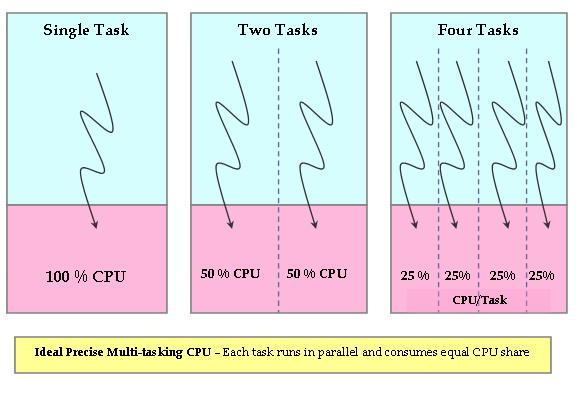
\includegraphics[width=0.7\columnwidth]{./pics/cpu0.jpg}
  \caption{Ideal CPU}
  \label{fig:Ideal CPU}
\end{figure}

Obviously, this ideal CPU is nonexistent, but the CFS tries to emulate such a processor in software. On an actual real-world processor, only one task can be allocated to a CPU at a particular time. Therefore, all other tasks wait during this period. So, while the currently running task gets 100\% of the CPU power, all other tasks get 0\% of the CPU power. This is obviously not fair. The CFS tries to eliminate this unfairness from the system. The CFS tries to keep track of the fair share of the CPU that would have been available to each process in the system.

\begin{figure}[H]
  \center
  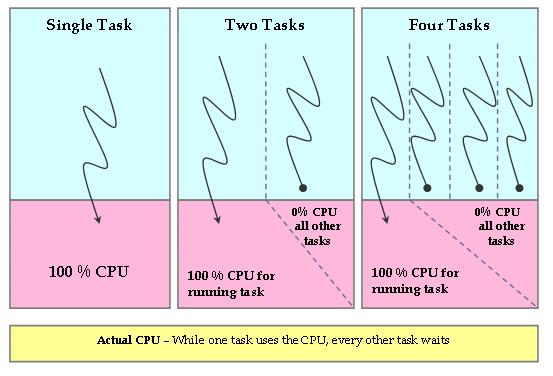
\includegraphics[width=0.7\columnwidth]{./pics/cpu1.jpg}
  \caption{Actual CPU}
  \label{fig:Actual CPU}
\end{figure}

The main idea behind the CFS is to maintain balance (fairness) in providing processor time to tasks. This means processes should be given a fair amount of the processor. When the time for tasks is out of balance (meaning that one or more tasks are not given a fair amount of time relative to others), then those out-of-balance tasks should be given time to execute.

To determine the balance, the CFS maintains the amount of time provided to a given task in what's called the virtual runtime. The smaller a task's virtual runtime—meaning the smaller amount of time a task has been permitted access to the processor—the higher its need for the processor. The CFS also includes the concept of sleeper fairness to ensure that tasks that are not currently runnable (for example, waiting for I/O) receive a comparable share of the processor when they eventually need it.

\begin{figure}[H]
  \center
  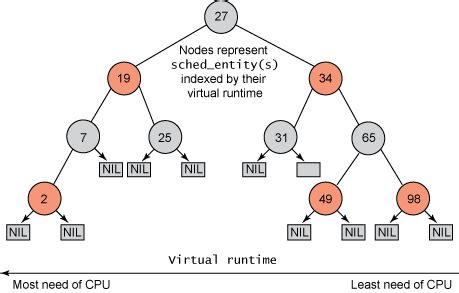
\includegraphics[width=\linewidth]{./pics/rbtsched.jpg}
  \caption{CFS Red-Black Tree}
  \label{fig:CFS Red-Black Tree}
\end{figure}

But rather than maintain the tasks in a run queue, as has been done in prior Linux schedulers, the CFS maintains a time-ordered red-black tree. A red-black tree is a tree with a couple of interesting and useful properties. First, it's self-balancing, which means that no path in the tree will ever be more than twice as long as any other. Second, operations on the tree occur in O(log n) time (where n is the number of nodes in the tree). This means that you can insert or delete a task quickly and efficiently.

With tasks (represented by \code{sched\_entity} objects) stored in the time-ordered red-black tree, tasks with the gravest need for the processor (lowest virtual runtime) are stored toward the left side of the tree, and tasks with the least need of the processor (highest virtual runtimes) are stored toward the right side of the tree. The scheduler then, to be fair, picks the left-most node of the red-black tree to schedule next to maintain fairness. The task accounts for its time with the CPU by adding its execution time to the virtual runtime and is then inserted back into the tree if runnable. In this way, tasks on the left side of the tree are given time to execute, and the contents of the tree migrate from the right to the left to maintain fairness. Therefore, each runnable task chases the other to maintain a balance of execution across the set of runnable tasks.

\subsubsection{\underline{Normal and Even Distributions for Processes}}

One very important aspect of the project is the decision on how to exactly generate processes. This seems like a strange problem, since processes are just processes, they don't even do anything in this project, but they play a key role. These jobs still have an impact on the overall performance of the program and it is not arbitrary how they are generated.

For instance, if all of the processes were the same, that would pose no variety in the global pool and thus every algorithm would have the same final output. True, each algorithm would be different, but with only one final result to show for it. This means that there must be a proper distribution made for the processes that are created, so that a real-life system is imitated as closely as possible. The question is, what type of distribution is most appropriate.

By first instinct, we would head towards a uniform distribution. Why? Because we want to treat every process as equal and reduce the algorithms being biased towards them. For instance, we don't want the \textbf{FCFS} procedure to outperform the other ones because it is having more short processes to execute, we want things to be evenly spread out. And although our intuition is heading for the right track, there is a problem. This approach is not realistic, as things in nature \textbf{do not} tend towards an even distribution. That is why we must have a good and realistic distribution in order to evaluate all of the processes properly in the end.

The underlying formula that is used for the \textbf{Gaussian Distribution} is

\begin{equation}
P(x) = \frac{1}{{\sigma \sqrt {2\pi } }}e^{{{ - \left( {x - \mu } \right)^2 } \mathord{\left/ {\vphantom {{ - \left( {x - \mu } \right)^2 } {2\sigma ^2 }}} \right. \kern-\nulldelimiterspace} {2\sigma ^2 }}}
\end{equation}

Of course this is provided \textit{as-is} from the standard \code{C++} implementations, and can be freely used for generating numbers.

But, there is a special use for a even distribution nonetheless. Namely, each process ID has to be unique and here we can create a generation algorithm that labels every process with a name that (probably) won't come twice.

Having said all of that, here is what the \textbf{Gaussian Distribution} is used for.

\begin{itemize}
\item Process Time to Live.
\item Process Number of IO Operations.
\item Process IO Operation duration.
\end{itemize}

From this, we can then pick the magic numbers which would go into each distribution. Because at this point, there isn't such a big deal as to how long (or short), each variable would be, a general estimate has been done. In the following table, we can see how the \textit{Mean} and \textit{Standard Deviation} play a role.

\begin{table}[H]
  \begin{center}
    \label{tab:Distributions of Process variables}
    \begin{tabular}{l|r|c}
      \toprule
       \textbf{Type} & \textbf{Mean $\mu$} & \textbf{Standard Deviation $\sigma$} \\
      \midrule
      Process TTL & 1000 ms & 270 ms \\
      IO TTL & 1500 ms & 150 ms \\
      Process-IO count & 10 & 2 \\
      \bottomrule
    \end{tabular}
    \caption{Distributions of Process variables}
  \end{center}
\end{table}

From this table we can see how the processes would be created and what to expect at each algorithm run. Each new process would most probably have a \code{time\_to\_live} somewhere between $730$ and $1270$ milliseconds, with about 10 \textit{IO} operations, each one taking about $1500$ milliseconds to execute. Thus the Gaussian plot will be like so:

\pgfmathdeclarefunction{gauss}{3}{%
  \pgfmathparse{1/(#3*sqrt(2*pi))*exp(-((#1-#2)^2)/(2*#3^2))}%
}

\begin{center}
  \begin{figure}[H]
    \begin{subfigure}[b]{1\textwidth}
      \begin{tikzpicture}
        \begin{axis}[
          domain=0:6,
          samples=100,
          ymin=0,
          axis lines*=left,
          xlabel=$process\_ttl_{ms}$,
          every axis y label/.style={at=(current axis.above origin),anchor=south},
          every axis x label/.style={at=(current axis.right of origin),anchor=north},
          height=5cm,
          width=16cm,
          xtick=\empty,
          ytick=\empty,
          enlargelimits=false,
          clip=false,
          axis on top,
          grid = major,
          hide y axis
          ]
          \addplot [very thick, codeblue] {gauss(x, 3, 1)};
          \pgfmathsetmacro\valueA{gauss(1,3,1)}
          \pgfmathsetmacro\valueB{gauss(2,3,1)}
          \pgfmathsetmacro\valueC{gauss(3,3,1)}
          \draw [gray] (axis cs:1,0) -- (axis cs:1,\valueA)
          (axis cs:5,0) -- (axis cs:5,\valueA);
          \draw [gray] (axis cs:2,0) -- (axis cs:2,\valueB)
          (axis cs:4,0) -- (axis cs:4,\valueB);
          \draw [gray] (axis cs:3,0)
          (axis cs:3,0) -- (axis cs:3,\valueC);
          \draw [yshift=1.4cm, latex-latex](axis cs:2, 0) -- node [fill=white] {$68\%$} (axis cs:4, 0);
          \draw [yshift=0.3cm, latex-latex](axis cs:1, 0) -- node [fill=white] {$95\%$} (axis cs:5, 0);

          \node[below] at (axis cs:1, 0)  {$460$};
          \node[below] at (axis cs:2, 0)  {$730$};
          \node[below] at (axis cs:3, 0)  {$\mu = 1000$};
          \node[below] at (axis cs:4, 0)  {$1270$};
          \node[below] at (axis cs:5, 0)  {$1540$};
        \end{axis}
      \end{tikzpicture}
      \caption{Process TTL Distribution}
    \end{subfigure}
  \end{figure}
\end{center}

The same would also be true for the other two variables in the table, just with different numbers.

\begin{figure}[H]
    \begin{subfigure}[b]{0.5\textwidth}
      \begin{tikzpicture}
        \begin{axis}[
          domain=0:6,
          samples=100,
          ymin=0,
          axis lines*=left,
          xlabel=$io\_ttl_{ms}$,
          every axis y label/.style={at=(current axis.above origin),anchor=south},
          every axis x label/.style={at=(current axis.right of origin),anchor=north},
          height=4cm,
          width=9cm,
          xtick=\empty,
          ytick=\empty,
          enlargelimits=false,
          clip=false,
          axis on top,
          grid = major,
          hide y axis
          ]
          \addplot [very thick, codeblue] {gauss(x, 3, 1)};
          \pgfmathsetmacro\valueA{gauss(1,3,1)}
          \pgfmathsetmacro\valueB{gauss(2,3,1)}
          \pgfmathsetmacro\valueC{gauss(3,3,1)}
          \draw [gray] (axis cs:1,0) -- (axis cs:1,\valueA)
          (axis cs:5,0) -- (axis cs:5,\valueA);
          \draw [gray] (axis cs:2,0) -- (axis cs:2,\valueB)
          (axis cs:4,0) -- (axis cs:4,\valueB);
          \draw [gray] (axis cs:3,0)
          (axis cs:3,0) -- (axis cs:3,\valueC);
          \draw [yshift=1.4cm, latex-latex](axis cs:2, 0) -- node [fill=white] {$68\%$} (axis cs:4, 0);
          \draw [yshift=0.3cm, latex-latex](axis cs:1, 0) -- node [fill=white] {$95\%$} (axis cs:5, 0);

          \node[below] at (axis cs:1, 0)  {$1200$};
          \node[below] at (axis cs:3, 0)  {$\mu = 1500$};
          \node[below] at (axis cs:5, 0)  {$1800$};
        \end{axis}
      \end{tikzpicture}
      \caption{IO TTL Distribution}
    \end{subfigure}
    %
    \begin{subfigure}[b]{0.5\textwidth}
      \begin{tikzpicture}
        \begin{axis}[
          domain=0:6,
          samples=100,
          ymin=0,
          axis lines*=left,
          xlabel=$\ \ \ \ \ io\_count$,
          every axis y label/.style={at=(current axis.above origin),anchor=south},
          every axis x label/.style={at=(current axis.right of origin),anchor=north},
          height=3cm,
          width=8cm,
          xtick=\empty,
          ytick=\empty,
          enlargelimits=false,
          clip=false,
          axis on top,
          grid = major,
          hide y axis
          ]
          \addplot [very thick, codeblue] {gauss(x, 3, 1)};
          \pgfmathsetmacro\valueA{gauss(1,3,1)}
          \pgfmathsetmacro\valueB{gauss(2,3,1)}
          \pgfmathsetmacro\valueC{gauss(3,3,1)}
          \draw [gray] (axis cs:1,0) -- (axis cs:1,\valueA)
          (axis cs:5,0) -- (axis cs:5,\valueA);
          \draw [gray] (axis cs:2,0) -- (axis cs:2,\valueB)
          (axis cs:4,0) -- (axis cs:4,\valueB);
          \draw [gray] (axis cs:3,0)
          (axis cs:3,0) -- (axis cs:3,\valueC);
          \draw [yshift=.83cm, latex-latex](axis cs:2, 0) -- node [fill=white] {$68\%$} (axis cs:4, 0);

          \node[below] at (axis cs:1, 0)  {$6$};
          \node[below] at (axis cs:3, 0)  {$\mu = 10$};
          \node[below] at (axis cs:5, 0)  {$14$};
        \end{axis}
      \end{tikzpicture}
      \caption{IO count per Process}
    \end{subfigure}
\end{figure}

The place where we can use a \textbf{Uniform Distribution} is for the generation of IDs. Each process is named with a random \textit{hexadecimal} value. The reason for doing this is because it simulates real processes in that each one is abstracted from what and where it came from. We care about what it does and how it is scheduled, an giving it a random name would be easiest to work with. This is done by generating a completely even number from $0 \rightarrow INT::MAX$ and then putting that number into a converter for \textit{hex} values. We get as an output a string that represents a unique name. The converter dose nothing more than converting that number int a hexadecimal value. The final output would look something like this.

\begin{table}[H]
  \begin{center}
    \label{tab:Process ID generation}
    \begin{tabular}{|c|}
      \toprule
       \textbf{Process ID} \\
      \midrule
      4b40 2e61 b88c 479c 831c d10e 9b54 bcfe a5f7 53f5 4d28 \\
      b5b2 73cd babd c920 5894 00a5 9bc8 5c6e 657c f561 ecd7 \\
      80ab 7d9b 7385 c52e 6d8a 242e 99ce fb27 0e9b f9d7 2a18 \\
      fa5b 3879 29df 2c15 9f48 3c6e 18cb cee3 d553 e15f 8dfe \\
      \bottomrule
    \end{tabular}
    \caption{Process ID generation}
  \end{center}
\end{table}

Of course there randomly generated processes hold the above-mentioned distributions for \textit{io/ttl/io-ttl}. They also have a priority, which is evaluated on each start for the different algorithms. This is shown by the colors they receive upon the start of execution.

\subsubsection{\underline{Data-structures}}

Because we are working with a lot of different types of classes, which interact heavily during every procedure, it's a good idea to see what each object does and in what type of structure does it integrate with. The classes that are involved with the process scheduling algorithms are as follows:

\begin{itemize}
\item \code{process} \\
  This class holds the data for each process. Instead of using a separate \code{PCB} block, which points to another \code{process} object, the project has been simplified for ease of use, thus it incorporates both these classes into one. The \code{process} class keeps track of its different statistics, which are then summarized in the end for the final evaluation. Each process has \textit{pre-defined} priority, or it can be evaluated upon creation, based on a normal distribution. Each process holds
  \begin{itemize}
  \item \textit{time to live} - \code{ttl}. The time each process it takes to execute completely.
  \item \textit{time of submission} - \code{tos}. The time at which the process starts executing.
  \item \textit{time of completion} - \code{toc}. The time at which the process finishes executing.
  \item \textit{turnaround time} - \code{tat}. The time between the time of submission and time of completion plus any \textit{IO} execution.
  \item \textit{waiting time} - \code{wait\_t}. The time a process spends in the \code{read\_queue} and is \textbf{not} executing.
  \item \textit{priority} - \code{prty}. The priority each process is assigned based on its execution time, or predefined from the start.
  \item \textit{IO operations} - \code{ioops}. The set of IO operations each process has.
  \item \textit{process id} - \code{id}. The unique ID that each process has.
  \end{itemize}
  In addition, this class also holds the data about its distribution, as specified in the previous section, in the for of constants.
\item \code{pool} \\
  This class used as a global pool, holding all of the different processes in their different states. Thus, there are \textit{queues} for \textbf{waiting processes}, \textbf{ready processes} and \textbf{done processes}. The pool itself is used as a general interface towards each process and its current structure. Because of this, it is much easier to perform operations on these queues, such as checking if they are empty, or clearing them, or even evaluating each process in a specific queue.
\item \code{scheduler}
  The scheduler is the structure that is responsible for controlling each executing algorithm. It interacts with the pool of processes, and executes them on the specified procedure. In addition to this, the scheduler also calculates \textit{both} the current and final \textbf{average waiting time} and \textbf{average turnaround time} of each algorithm, based on the passed processes. The class also specifies additional constants, like an \code{ALPHA} value for future predictions, and \code{TIME\_QUANTUM} for equal process execution. \\
  The general steps of execution are like this:
  \begin{algorithm}[H]
    \caption{Generic Scheduling}\label{generic sched}
    \begin{algorithmic}[1]
      \Ensure $globals:=reset()$
      \Ensure $processes \gets evaluated()$
      \While {$pool \ne empty$}
      \State $screen.update()$
      \If {$process \gets IO$}
      \State \Call{execute}{$\frac{time\_q}{2}$}
      \State $dispatcher::interrupt$
      \Else
      \State \Call{execute}{$time\_q$}
      \State $dispatcher::context\_switch$
      \EndIf
      \State $awt \gets calculate()$
      \EndWhile
      \State $screen.show\_summary()$
    \end{algorithmic}
  \end{algorithm}
\item \code{dispatcher} \\
  The dispatcher structure is used to work on the \code{context\_switch}-es and \code{interrupt}s. Thus, it takes every process that has finished executing its designated time and performs either one of the two operations. When it does a \code{context\_switch}, it goes through the procedure of \(save\_state() \rightarrow restore\_state()\). When the state is saved, the current process is updated and then goes to the restore step. If the process is done, it is finalized and pushed to the \code{done\_queue}, then the screen is updated and the reference to the next process is taken. If there is an interrupt, which occurs on any \textit{IO}, then a separate \code{thread} is created and \textit{detached} from the \textbf{parent process}. The new thread then takes the specific process and executes the next IO operation that it's waiting. After its completion, the process is returned back to the \textbf{end} of the \code{ready\_queue}.
\end{itemize}

Having this general idea of how all these classes are constructed and what they do, we can have a clearer picture of the created data-structures that arise.

There are three vector, treated as queue, working on the basis of \textbf{FIFO}. The queues are the \code{ready\_queue}, the \code{waiting\_queue}, and the \code{done\_queue}. The \code{ready} vector holds all of the processes that are in the \code{READY} state, which means that they are ready to execute their next CPU Burst(s). The \code{wait} vector is for processes that have interrupted the algorithm and have been sent to do IO. Generally, a process can interrupt the system because its part of its natural life span, but it can also do that when it wants to request IO and has to be sent to do that operation. In this project, only IO operations are considered to raise such interrupts, due to the fact that the rest of the operations would not matter so much to the general performance. These processes are thus labeled as being in \code{WAITING} state and will return to the back of the \code{ready\_queue} once they are done with their other procedure(s). The \code{done} vector is the one that holds all of the processes that have \textit{completely} finished their execution time and don't have any more work to do. These vectors are not parallel, but rather hold the same process, just in different times and quantities. The whole pool of processes is the sum of the processes found in the \code{ready\_queue} and the \code{waiting\_queue}. The pool is considered empty when \textbf{both} these queues do not have any process in them. This means that the \code{waiting\_queue} can have a size of $0$, while the ready one has all of the processes in it. And vise versa, the \code{ready\_queue} can be completely empty while all of the processes are doing some sort of IO (although this situation is highly unlikely).

\subsubsection{\underline{User Interface}}

The \textit{UI} of this project takes an alternative approach. Because the main focus of the application is towards algorithm execution, the interface tries to be as simple as possible and to convey the idea on what is happening in the easiest manner possible. For this reason, all of the UI is created inside of a \textit{terminal emulator}, with additional graphics added. With the help of the \code{ncurses} library, used for graphics in the terminal, the final product looks nice and easy to understand without being too flashy.

The structure of \textit{UI} is as follows: 4 main panels, each one holding information for the processes and the currently executing algorithm. Let's go through them one by one:

\begin{itemize}
\item \textbf{ALGORITHM} panel - This panel is used to display the currently running process and its different data. Things like its priority, \code{ttl}, and ID, are shown at the top. Upon each algorithm completion, a summary is displayed below, indicating the \textit{Average Waiting Time} and \textit{Average Turnaround Time} for that algorithm. In addition to this, the name of the used algorithm together with the number of processes is displayed as well.

  \begin{figure}[H]
    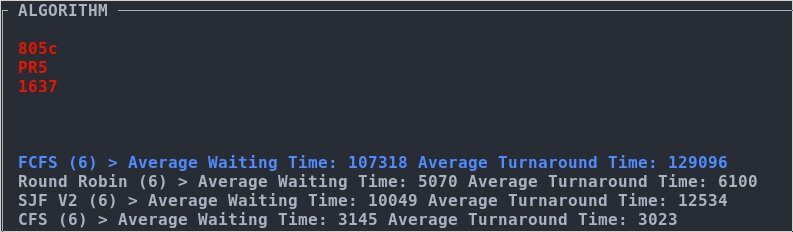
\includegraphics[width=\linewidth]{./pics/alg.jpg}
    \caption{Algorithm Panel}
    \label{fig:Algorithm Panel}
  \end{figure}

  Here we can see the output of several algorithms with a process running. We can see how the processes is colored into a priority and how the summaries of the previous algorithms are shown to the user. The most recently run algorithm is also colored so it makes it easier to remember which is the most recent piece of data.

  On the very bottom of this panel, there are two miniature windows. Both of them depict the graph of the \textit{Waiting Time} and \textit{Turnaround Time} in terms of \textbf{amount of time} (on the $y-axis$) and number of processes (on the $x-axis$). That is, at each CPU Burst rotation, the graph shows what are the current averages. This gives an idea on how the algorithm is performing over time. When it comes to comparing, these graphs will make it easier for further evaluation and records keeping.

  \begin{figure}[H]
    \centering
    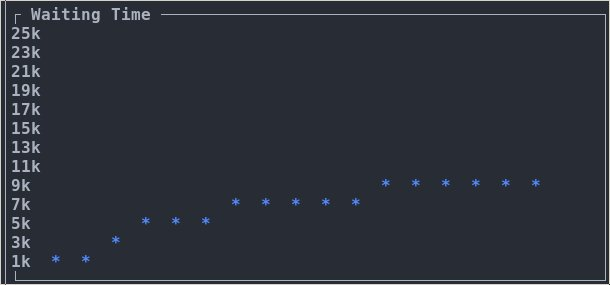
\includegraphics[width=0.75\columnwidth]{./pics/awt.jpg}
    \caption{Waiting Time Panel}
    \label{fig:Waiting Time Panel}
  \end{figure}

  Here is the screen for the graphical output of the average waiting time. We can see that on the left we have a scale that depicts the running time in milliseconds and it also plots the dots in the window. In this specific case, we can see the graph being very close to a logarithmic function. This is a big help when we are evaluating the algorithms in the end.

\item \textbf{PROCESS} panel - This panel holds all of the processes that are in the \code{ready\_queue}. When a job jumps from doing CPU Bursts to doing IO operations, it jumps out of this panel, does its thing, and comes back inside again an the end of queue. When each CPU Burst finish, all of the processes do a rotation with one to the left, where the leftmost process will be the next one to execute. If a process is done, however, then it is popped out of the panel and inserted into the next one.

  \begin{figure}[H]
    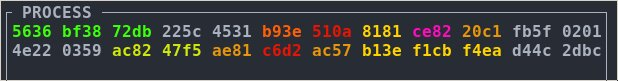
\includegraphics[width=\linewidth]{./pics/prcs.jpg}
    \caption{Process Panel}
    \label{fig:Process Panel}
  \end{figure}

  In this screen we can see how the different processes and mix of processes are all in the ready queue. This means that all of these are either about to be executed or are being executed in the moment. We can see that some of the processes are already with a pre-defined priority, while the white ones will get theirs as soon as the algorithm is started.

\item \textbf{DONE} panel - As mentioned above, this is the place where all of the done processes are held. The inserted processes are in the order of their completion.

  \begin{figure}[H]
    \centering
    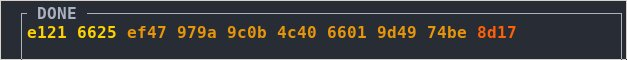
\includegraphics[width=\linewidth]{./pics/doneq.jpg}
    \caption{Done Panel}
    \label{fig:Done Panel}
  \end{figure}

  In this panel we can see a set of processes that have already finished execution and are put in the order by which they have finished.

\item \textbf{LEGEND} panel - This is the final panel and it holds information for all of the commands the user can send to the program. This makes working with the application easier. On the top, the different priorities are shown, together with the key that will spawn a process with that priority. There are 7 in total, starting form 0, all the way up to priority 6. There is an additional key that creates random processes, that will not have a priority, but that will be evaluated by the algorithm at execution time. Below this, the legend also shows each of the implemented processes in the system plus the key that will start executing it. When a procedure is started, below it, a text will appear which will explain what are its features and what it does. That way, the learning and evaluation process is made easier on the user.

  \begin{figure}[H]
    \centering
    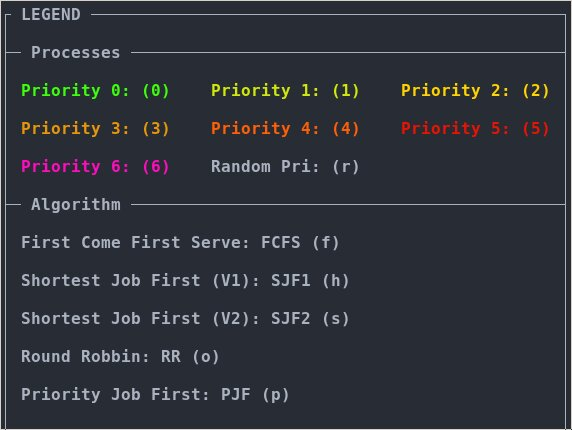
\includegraphics[width=0.75\columnwidth]{./pics/legend.jpg}
    \caption{Legend Panel}
    \label{fig:Legend Panel}
  \end{figure}

  The legend panel color coded and we can see that in the brackets, next to each procedure, there is a character that will initiate it. Then, we can see how there are two sub-panels, one for the processes and one for the algorithms. This makes it exactly clear to the user what are the functionalities of the application.

  On top of everything, there is also additional information that is given for each algorithm that is being currently run. This information can be used to understand what is happening currently on the screen and to also make it easier for any pedagogical lessons.

  \begin{figure}[H]
    \centering
    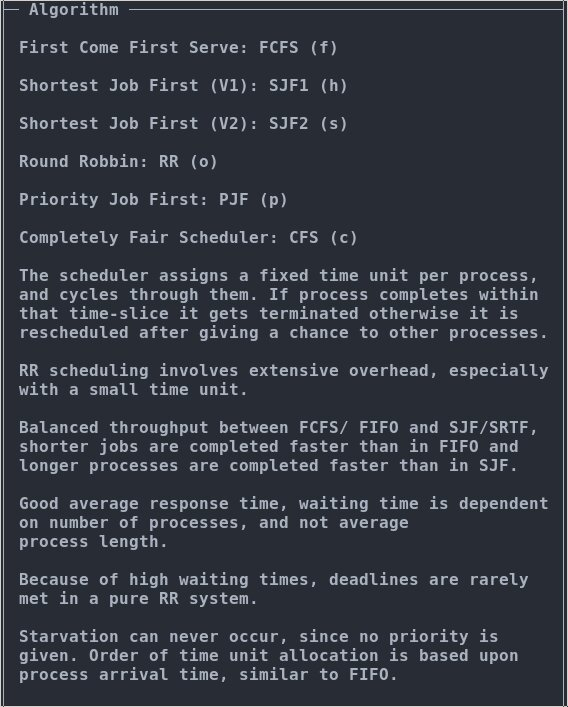
\includegraphics[width=0.65\columnwidth]{./pics/legenddata.jpg}
    \caption{Legend Info Panel}
    \label{fig:Legend Info Panel}
  \end{figure}

  Here we can see that the text is placed in the free area of the application in the Legend panel and is currently explaining about the Round Robin algorithm. This looks both nice visually and is helpful at the same time.

\end{itemize}

Because the user interface has to also have some form of input, we must also accommodate to the fact that we must enter some data into the application. This means that we must parse some input from the user to the different processes into the app. This is done through the ncurses library, which allows for inputs. With the \code{getch()} method, which returns a number representation of the pressed character from the keyboard, we can see what the user has pressed. By following the legend and having the input given by the user, we can see what is needed to be done in the app. For instance, we might start executing some algorithm or we might create a specific process.

The legend for the different accepted types of input is as follows:

\begin{itemize}
\item \code{0} to \code{6}. Pressing one of the numbers from 0 to 6 will create a certain type of a process, which is based on a priority. The priority on each of the button presses is expressed by a graphical color, indicated in the legend. When a process is created this way, the process with its ID is added to the ready queue and is printed with the priority color immediately.
\item \code{r}. When this key is pressed, then a new type of process is created - a random one. Based on the aforementioned rules for process distribution, a new process is added to the ready queue and is colored in white, because then the algorithm will evaluate the process priority. It is completely possible for a user to both combine and mix random and pre-defined processes in the ready queue, which would cause the queue to be filled with colored and non-colored processes.
\item \code{f}. When pressing the F key, we start working with the different algorithms. In this case, the FCFS algorithm would start executing on the filled ready queue. This means that we will start seeing how the processes we just created will be treated by this algorithm.
\item \code{h}. As with the previous key, this will start the SJF method 1 algorithm.
\item \code{s}. This is the SJF method 2 implementation.
\item \code{o}. This is the Round Robin algorithm key.
\item \code{p}. This is the Priority First scheduler.
\item \code{c}. This is the Completely Fair Scheduler in action.
\end{itemize}

\subsubsection{\underline{Software Architecture}}

The Software Architecture of the project can be seen as one of the following: \textit{MVC}, \textit{Monolithic}, \textit{Event-driven}, or \textit{Procedural}. If we look at the project as a \textit{Monolithic}, we can say that it encapsulates itself into a \textit{single-tiered} software application in which the user interface and data access code are combined into a single program from a single platform. A monolithic application is self-contained, and independent from other computing applications. The design philosophy is that the application is responsible not just for a particular task, but can perform every step needed to complete a particular function. On the other hand, were we to look at it through the perspective of the \textit{Event-driven} design, we can see how it follows a pattern promoting the production, detection, consumption of, and reaction to events. An \textit{event} can be defined as \textit{"a significant change in state"}. For example, when a \textbf{process} \code{ttl} is completely done, it changes state from \code{RUNNING} $\rightarrow$ \code{DONE}. And again, if we are to look at the project from the standpoint of a \textit{Procedural} system, we would see that it follows a certain set of rules, which in the end, produce an output that can be interpreted and evaluated for further work. As an example, we would be able to see how the \textbf{SJF} algorithm performs under long processes.

\bigskip

\textbf{\underline{MVC}}

The Model View Controller (usually known as MVC) is an architectural pattern commonly used for developing user interfaces that divides an application into three interconnected parts. This is done to separate internal representations of information from the ways information is presented to and accepted from the user. The MVC design pattern decouples these major components allowing for efficient code reuse and parallel development.

The Model View Controller approach in this project can be seen as the following way. First, we can check what is the Model of the application. This is the part where the data is stored and is handled by the business logic. The central component of the pattern. It is the application's dynamic data structure, independent of the user interface. It directly manages the data, logic and rules of the application. A large part of the app is in the Model section, because it is handling and working with a lot of algorithmic data. So we can consider that the Dispatcher, Scheduler, the Red-Black tree, the Process Poll, Processes, etc. Because all of this data is working in the background and we just see its visualization, we can put it in the Model.

\subsubsection{\underline{Security Features}}

\section{\underline{Implementation}}

This software is developed entirely with the \code{C++} programming language. All of the implementation uses the \code{C++ 11} standard (and up). The \code{C++ 11} standard and all of its follow-up additions, all the way up to \code{C++ 20}, have great benefits to creating modern, safe, and easy to manage software. Many functionalities introduced since \code{C++ 11} have been used to create this project. Most noticeably, the use of lambda functions, collection manipulators, threads and mutexes, and many more, play a key role.

In addition to this, the famous library \code{ncurses} is used in order to make working with terminal emulators easier. \code{ncurses} provides an \code{API} for manipulating the graphics and output of the terminal. Since this is an application, based on working with a terminal emulator, such a library would be of great help. The specific terminal that was used to test and run the application is \code{xterm}, but this was also tested on \code{gnome-terminal}.

The operating system used to create the software is \code{Arch Linux}, with additional testing environment under \code{Fedora 29}.

\section{\underline{Testing}}

\section{\underline{Result and Conclusion}}

In the end we have to compare all this information. We would expect that in theory, some of the algorithms would be significantly slower than others.

In this table, we see how we are comparing several algorithms, based on the number of processes that are submitted to the queue.

\begin{center}
  \begin{tabular}{l|c|c|r}
    \multicolumn{4}{c}{FCFS} \\
    \toprule
    \textit{Num Processes} & \textbf{Exec Time}$_{ms}$ & \textbf{Wait Time}$_{ms}$ & \textbf{Turnaround Time}$_{ms}$ \\
    \midrule
    20 & 19746 & 9713 & 1007 \\ \hline
    50 & 50293 & 24186 & 971 \\ \hline
    100 & 101362 & 51690 & 1029 \\ \hline
    200 & 200948 & 102545 & 1032 \\
    \bottomrule
    \toprule
    \multicolumn{4}{c}{SJF1} \\
    \toprule
    \textit{Num Processes} & \textbf{Exec Time}$_{ms}$ & \textbf{Wait Time}$_{ms}$ & \textbf{Turnaround Time}$_{ms}$ \\
    \midrule
    20 & 19814 & 8542 & 1057 \\ \hline
    50 & 49986 & 18360 & 959 \\ \hline
    100 & 99770 & 43420 & 1047 \\ \hline
    200 & 200805 & 82409 & 1015 \\
    \bottomrule
    \toprule
  \end{tabular}
\end{center}
\newpage
\begin{center}
  \begin{tabular}{l|c|c|r}
    \multicolumn{4}{c}{SJF2} \\
    \toprule
    \textit{Num Processes} & \textbf{Exec Time}$_{ms}$ & \textbf{Wait Time}$_{ms}$ & \textbf{Turnaround Time}$_{ms}$ \\
    \midrule
    20 & 73043 & 38126 & 34787 \\ \hline
    50 & 188321 & 98706 & 78400 \\ \hline
    100 & 368691 & 202500 & 159449 \\
    \bottomrule
    \toprule
    \multicolumn{4}{c}{RR} \\
    \toprule
    \textit{Num Processes} & \textbf{Exec Time}$_{ms}$ & \textbf{Wait Time}$_{ms}$ & \textbf{Turnaround Time}$_{ms}$ \\
    \midrule
    20 & 20593 & 17512 & 18125 \\ \hline
    50 & 50411 & 45391 & 45254 \\ \hline
    100 & 192607 & 81059 & 79558 \\
    \bottomrule
    \toprule
  \end{tabular}
\end{center}

\section{\underline{References}}

\end{document}